\chapter{Likelihood Point Estimation}
\minitoc
\section{Introduction}
Diffusion Maps in \cref{chap:diff_maps} provide a good initial point estimate for fitting GIRG node locations to a real graph. The actual data likelihood, $p(G | \theta)$, however, is what we'd truly like to maximise. As in \cite{garcia2019mercator} we can use the likelihood to do a further refinement of point locations, although finding anything like a global optimum is infeasible for all but tiny graphs.

We first tried a Markov Chain Monte Carlo (MCMC) approach to not just improve $p(G | \theta)$ but also, in theory provide an estimate of the posterior distribution of $p(\theta | G)$. While effective, it was quite slow, so we later shifted to using a direct $p(G | \theta)$ optimisation with rounds of point updates, in order from highest to lowest degree node, inspired by \cite{garcia2019mercator}.

\section{MCMC Formulation}
MCMC is a method in the bayesian framework of a parametric generative model. Datapoints $z$ are generated by first sampling $\theta \sim p(\theta)$ from a prior, and then generating from the model $z \sim p(z | \theta)$. In our case of our node specific fitting GIRG GGM, $\theta = (\alpha, c, \{w_u\}_{u \in V}, \{x_u\}_{u \in V})$, and we focus in particular on the locations $x_u$. $z$ for us is one real graph instance $G$.

The posterior likelihood $p(\theta | z) = \frac{p(z | \theta) p(\theta)}{p(z)}$ is infeasible to compute due to the normalising factor $p(z)$. MCMC instead uses the non normalised $Q(\theta) = p(z | \theta) p(\theta)$ which can be evaluated, to set up a Markov Chain (MC) with states $\theta \in \Theta$, and transition probabilities derived from $Q(\theta)$.
In particular we will use a Metropolis-Hastings style MC.
With a proper MC state transition probability $p(\theta \to \theta')$, we can perform a random walk on the MC state space that converges in the limit to the posterior distribution $\theta \sim p(\theta | z)$. If the jth step of the random walk yields $\theta^j$, given sufficient burn in and spacing, we can sample $\theta^{j_1}, \theta^{j_2}, ...$ from the posterior. We will be content with just one posterior sampled $\hat{\theta}$ (NB not a maximum likelihood estimator), and use this to evaluate our overall GIRG model fit to the real graph.

We transition $\theta \to \theta'$ with a Gibb's sampling approach. This means breaking down $\theta$ into subcomponents $\theta_i$, randomly choosing one to propose a new state for, i.e. $\theta' = (\theta'_i, \theta_{-i})$, and using the $Q_i(\theta_i)$ instead of $Q(\theta)$ - i.e. just the marginal non-normalised posterior.
In our case $Q(\theta) = p(G | \theta) p(\theta)$, so the uniform prior $p(\theta)$ can be dropped everywhere as $p(\theta) = 1\; \forall \theta$, and then $p(G | \theta) = \prod_{(u,v) \in {V \choose 2}} p(e(u,v) | w_u, w_v, x_u, x_v, \alpha, c, G)$.
This lends well to Gibb's sampling - we need concentrate only on $Q_u(\theta_u) = \prod_{v \neq u} p(e(u,v) | ...)$.

% Key elements of the MCMC approach are 1. burn in time, and 2. proposal distribution. 

Burn in time can be quite long. With the GIRG model, the natural initialisation for $x_u$ would be to follow the prior $x_u \sim U([0, 1]^d)$. By using a diffusion map embedding initialisation this can be greatly reduced.

The proposal distribution should be designed to maximise chances of acceptance. It seemed reasonable to stochastically propose either a small local perturbation, or a random jump to anywhere in the cube, with some probability of either (we elected for 70\% small perturbation). A random uniform jump is useful to try and find a completely new location for $x_u$ that could suit (hopefully near to its neighbours) - in fact another good proposal would be to randomly choose a neighbour $v \sim u$, and move $x_u$ to a random offset of $x_v$. A small perturbation $x_u' = x_u + \epsilon$ is good as assuming $x_u$ has high likelihood, somewhere nearby might have even higher.

\paragraph{Acceptance probability} in the Metropolis-Hasting's algorithm
\begin{align}
  A(x_u', x_u) &= \min \left (1,\;\;  \frac{p_{prop}(x_u | x_u') p(G | x_u') p(x_u')}{p_{prop}(x_u' | x_u) p(G | x_u) p(x_u)}\right )
  \\
  &= \min \left (1,\;\;  \frac{p(G | x_u')}{p(G | x_u)} \right )
  \\
  & \text{as $p_{prop}$ is symmetric and $p(x) = 1\; \forall x$}
\end{align}

\begin{comment}
\section{Bayes Factor likelihood comparisons}
\begin{enumerate}
    \item Using one MCMC posterior sample of $\{x_u\}_{u \in V}$ and maximum likelihood estimates $\hat{\alpha}, \hat{c}, \hat{w}_u$, we estimate the likelihood $p(\cG_{\GIRG} | G)$, and can perform a comaprison $p(\cG_{\GIRG-1d} | G)$ vs $p(\cG_{\GIRG}-2d | G)$ vs $p(\cG_{CL} | G)$ etc.
    \item Results show that $p(\cG_{\GIRG}-1d | G)$ is better than 2D, 3D GIRGs, but not as good as Chung-Lu
    \item Results show that simply introducing a failure rate of $0.5$ onto the GIRGs (unfortunately not correcting for LCC), the model probabiltiy estimate for 1D GIRG then beats out Chung-Lu (all copyweights)
\end{enumerate}


What the heck is Bayes Factor anyway?

Apparently it's basically comparing $P(M_1 | D)$ and $P(M_2 | D)$. In our case $M_1, M_2$ is e.g. 1D GIRG vs 2D GIRG, and $D$ the data is just one graph instance. We have some prior of $P(M_1)$ vs $P(M_2)$, e.g. 50-50, or some kind of decaying $1D \GIRG > 2D \GIRG > 3D \GIRG > \dots$.

Then the comparison is $P(M_1 | D) = \frac{P(D | M_1) P(M_1)}{P(D)}$. I.e. the ratio $\frac{P(M_1 | D)}{P(M_2 | D)}$ is the ratio $\frac{P(D | M_1) P(M_1)}{P(D | M_2) P(M_2)}$.

We will ignore the priors $P(M_1), P(M_2)$, for now, and focus on the likelihoods $P(D | M_1), P(D | M_2)$. In our case if $M_1$ is a 1D GIRG, and we've decided to fix e.g. $\alpha, e, \{w_u\}_{u \in V}$, and just vary $\theta = c, \{x_u\}_{u \in V}$, then we could monte-carlo sample $\theta \sim p(\theta)$ from the prior to get an estimate, $P(D | M_1) = P(G) = \int_\theta P(G | \theta) p(\theta) d\theta$, where we drop the $| M_1$ as we've fix into the 1D GIRG universe.

This seems inefficient. Instead we can sample $\theta \sim P(\theta | G)$ from the posterior using MCMC, and then evaluate  

\begin{align*}
    1/P(G) 
        &= \int_\theta \frac{1}{P(G)} P(\theta) d\theta
        \\
        &= \int_\theta \frac{P(\theta, G)}{P(G)} \frac{1}{P(\theta, G)} P(\theta) d\theta 
        \\
        &= \int_\theta P(\theta | G) \frac{P(\theta)}{P(\theta, G)} d \theta
        \\
        &= \int_\theta P(\theta | G) \frac{1}{P(G | \theta)} d\theta
        \\
        &= E_{\theta \sim \theta | G} \left [ \frac{1}{P(G | \theta)} \right ]
        % &= \int_\theta P(\theta) P(G | \theta) d\theta
        % \\
        % &= \int_\theta P(\theta) \frac{P(\theta | G)}{P(\theta | G)} P(G | \theta) d\theta
        % \\
        % &= \int_\theta \frac{P(G, \theta)}{P(\theta | G)} P(\theta | G) d\theta
        % \\
        % &= \int_\theta \frac{P(G | \tehta) | \theta}
\end{align*}

The good news is that while MCMC sampling from $P(\theta | G)$, it seems that the likelihood $P(G | \theta)$ is relatively consistent.

TODO think through more penalisation of models by parameter count. Does this $P(G)$ calculation take this into account already? I.e. a high parameter count model can fit many different $G$, so although $G$ is more "plausible" under a higher count model, there are also more alternative outcomes $G'$ so as to dilute the probability?
\end{comment}

\subsection{MCMC Likelihood comparison of GIRG vs CL fit to real graph}
How well do the converged MCMC points do at replicating the real graph? As suggested in the classification comparison framework, Chung-Lu model is a good non-geometric null hypothesis to compare against - i.e. we hope the MCMC fit GIRG model will do better than Chung-Lu. It's also interesting to see how large dimension $d$ GIRG is necessary for a good fit.

As a first sanity check, we compare the MCMC fit $\hat{\theta}_{\GIRG}$ to the more simply fit (copy degrees as weights) Chung-Lu parameters $\hat{\theta}_{CL}$, by comparing $p(G | \hat{\theta}_{\GIRG}, \cG_{\GIRG})$ vs $p(G | \hat{\theta}_{CL}, \cG_{CL})$. 

For most of the facebook graphs however, $p(G | \hat{\theta}_{\GIRG}, \cG_{\GIRG}) < p(G | \hat{\theta}_{CL}, \cG_{CL})$, despite GIRGs having more parameters / flexibility to fit $G$!

The GIRG model is far too confident about edges, giving $p_{uv} \approxeq 1$ for small $\norm{x_u - x_v}$ and $p_{uv} \approxeq 0$ for large $\norm{x_u - x_v}$. Hence a mistake on a few edges can lead to a large penalisation in likelihood. The Chung-Lu model is much more forgiving, with all probabilities more medium sized. 

% by evaluating the likelihood $p(G | \hat{\theta}, \cG)$ for both models. We expect that the GIRG model will do better, as it has more parameters to fit, and is more flexible.
% we can sample a $\hat{\theta}_{\GIRG}$ (not MLE but still pretty good) as from the posterior $\theta_{\GIRG} | G$ with MCMC, and more simply fit a $\hat{\theta}_{CL}$. Given that the 1D GIRG is a more parametrised model, it would be total failure if it didn't reproduce the given graph better. For most of the facebook graphs however, $p(G | \hat{\theta}_{\GIRG}, \cG_{\GIRG}) < p(G | \hat{\theta}_{CL}, \cG_{CL})$!
% The GIRG model is far too confident about edges, giving $p_{uv} \approxeq 1$ for small $\norm{x_u - x_v}$ and $p_{uv} \approxeq 0$ for large $\norm{x_u - x_v}$. Hence a mistake on a few edges can lead to a large penalisation in likelihood. The Chung-Lu model is much more forgiving, with all probabilities more medium sized. 

One reasonable tweak is to introduce a failure rate $0 \leq f \leq 1$ to the GIRG model: 
% $p_{uv} = (1-f) \min( ... )$
\begin{equation}
  p_{uv} = (1 - f) \min \left \{ 
    1,
    c \left (
        \frac{w_u w_v / W}{\norm{x_u - x_v}^d}
    \right )^\alpha    
\right \}
\end{equation}
For a social network this means that two highly similar people are not guaranteed/forced to be friends. Indeed there may be a very like-minded person who lives next door to you that you've never met, or had no opportunity / free time to properly get to know.

A failure rate will lower the impact of short non-edges (mistakenly predicted high probability of edge), but for long edges (mistakenly predicted low probablity of edge) we need a baseline edge probability to prevent $p_{uv}$ being too small. A simple fix is to mixin the Chung-Lu model - i.e. let 
\begin{equation}
  p_{uv} = \eta \; p_{uv}^{CL} + (1 - \eta) \; p_{uv}^{GIRG}
\end{equation}
for $0 \leq \eta \leq 1$. This should not be seen strictly as an ensemble of models or gross addition to the number of parameters of the GIRG model, as the GIRG model already contains fit node weights $(\hat{w}_u)_{u \in V}$. The mixin parameter $\eta$ does also help a lot on short non-edges similarly to failure rate $f$, but it could still be good to have both as even the Chung-Lu model can demand an edge $u \sim v$ with high probability if $w_u, w_v$ are both very large - though this is very rare.

The intuitive social network interpretation of Chung-Lu mixin is that it allows for some "random" friendships.


With these two new parameters $f, \eta$, the augmented GIRG model does have a higher specific fit likelihood than the Chung-Lu model: $p(G | \hat{\theta}_{GIRG}, \cG_{GIRG}) > p(G | \hat{\theta}_{CL}, \cG_{CL})$. In a holistic MCMC setup these two parameters could also have a prior and be sampled from the posterior, but for simplicity we set them to $f=0.3, \eta=0.5$. See \cref{fig:mcmc_runs} for some likelihood convergence curves on some example graphs.


% TODO Must input graphs here hold up


\begin{figure}
  \centering

  \begin{subfigure}{0.49\textwidth}
    \centering
    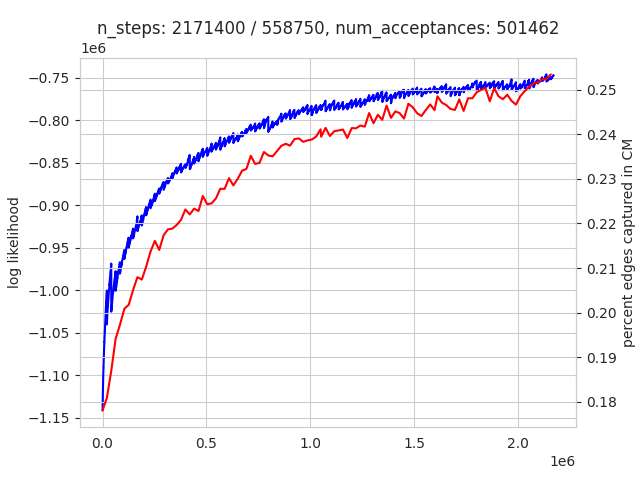
\includegraphics[width=\linewidth]{figures/MCMC_plots/socfb-Amherst41-1d.png}
    \caption{Amherst41 $d=1$}
  \end{subfigure}
  \hfill
  \begin{subfigure}{0.49\textwidth}
    \centering
    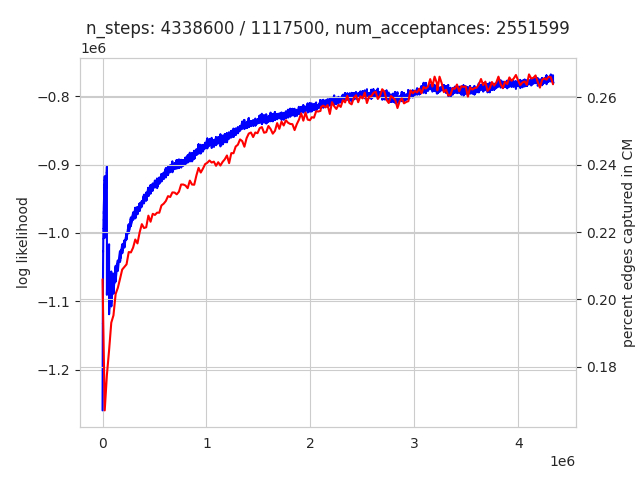
\includegraphics[width=\linewidth]{figures/MCMC_plots/socfb-Amherst41-2d.png}
    \caption{Amherst41 $d=2$}
  \end{subfigure}

  \vspace{1em}

  \begin{subfigure}{0.49\textwidth}
    \centering
    \includegraphics[width=\linewidth]{figures/MCMC_plots/socfb-Trinity100-1d.png}
    \caption{Trinity100 $d=1$}
  \end{subfigure}
  \hfill
  \begin{subfigure}{0.49\textwidth}
    \centering
    \includegraphics[width=\linewidth]{figures/MCMC_plots/socfb-Trinity100-2d.png}
    \caption{Trinity100 $d=2$}
  \end{subfigure}

  \vspace{1em}
  \begin{subfigure}{0.49\textwidth}
    \centering
    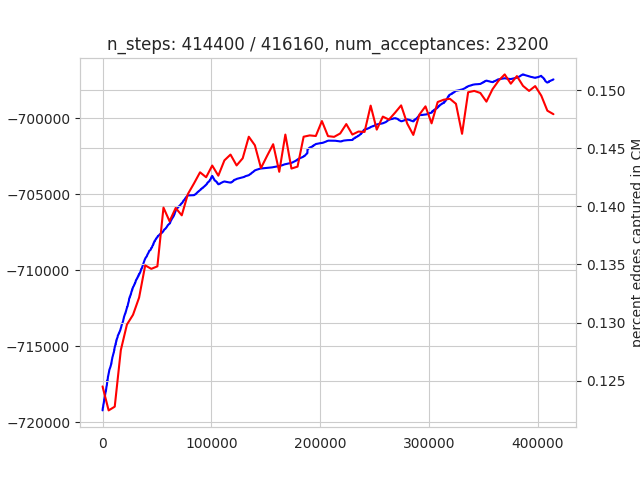
\includegraphics[width=\linewidth]{figures/MCMC_plots/socfb-Hamilton46-1d.png}
    \caption{Hamilton46 $d=1$}
  \end{subfigure}
  \hfill
  \begin{subfigure}{0.49\textwidth}
    \centering
    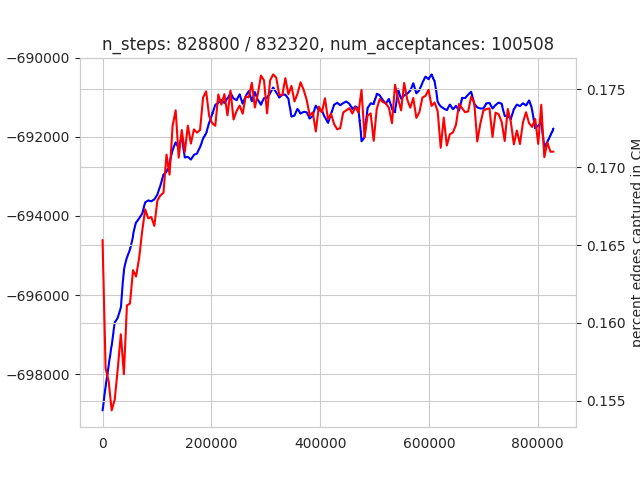
\includegraphics[width=\linewidth]{figures/MCMC_plots/socfb-Hamilton46-2d.png}
    \caption{Hamilton46 $d=2$}
  \end{subfigure}

  % \vspace{1em}
  % \begin{subfigure}{0.49\textwidth}
  %   \centering
  %   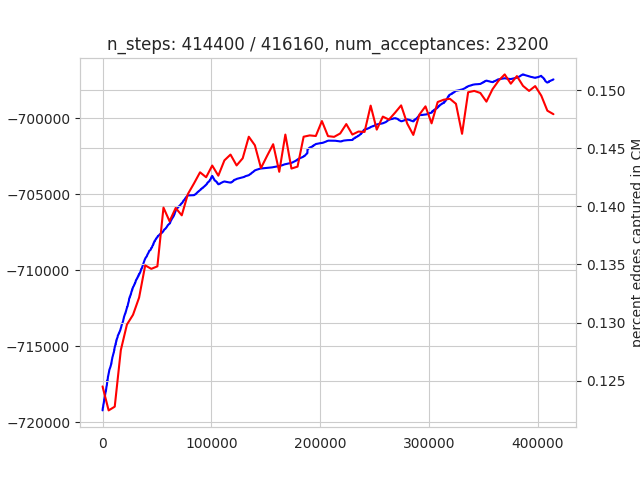
\includegraphics[width=\linewidth]{figures/MCMC_plots/socfb-Hamilton46-1d.png}
  %   \caption{$d=1$}
  % \end{subfigure}
  % \hfill
  % \begin{subfigure}{0.49\textwidth}
  %   \centering
  %   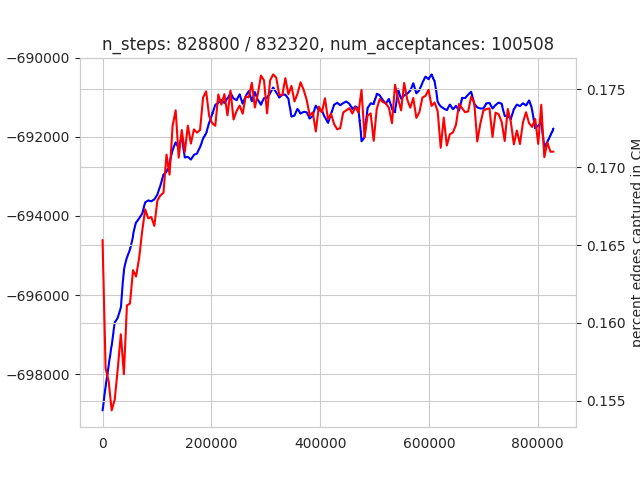
\includegraphics[width=\linewidth]{figures/MCMC_plots/socfb-Hamilton46-2d.png}
  %   \caption{$d=2$}
  % \end{subfigure}

  % \vspace{1em}
  % \begin{subfigure}{0.49\textwidth}
  %   \centering
  %   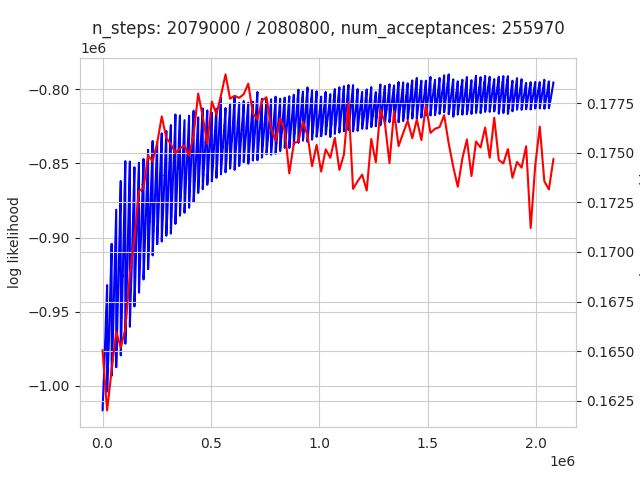
\includegraphics[width=\linewidth]{figures/MCMC_plots/socfb-Hamilton46-3d.png}
  %   \caption{$d=1$}
  % \end{subfigure}
  % \hfill
  % \begin{subfigure}{0.49\textwidth}
  %   \centering
  %   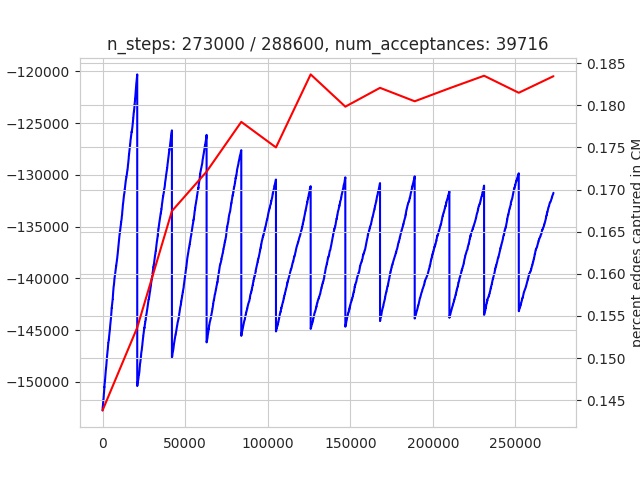
\includegraphics[width=\linewidth]{figures/MCMC_plots/socfb-Reed98-1d.png}
  %   \caption{$d=2$}
  % \end{subfigure}

  % \vspace{1em}


  \caption{MCMC runs for socfb-Amherst41, sofcb-Trinity100, socfb-Hamilton46 with failure rate $0.3$ and Chung-Lu Mixin rate $0.5$, with a cube GIRG model. Log likelihood wise, Amherst 1D GIRG does best; for Bowdoin it's 2D GIRG.
  x axis is number of steps; left y axis (blue curve) is log likelihood; right y axis (red curve) is PEC}
  \label{fig:mcmc_runs}
\end{figure}

\subsection{Percent Edges Captured Metric Comparison}
Another simple framework to compare quality of fit without taking into account increased parametrisation is to analyse the "accuracy" on successfully producing edges / non-edges.

Our MCMC posterior is constrained by directly fitting $\hat{c}$ to produce a similar number of edges $|E|$ as in the real graph. Hence in the standard classification confusion matrix
\begin{equation}
  \begin{array}{|c|c|}
    \hline
    TP & FN \\
    \hline
    FP & TN \\
    \hline
    \end{array}
\end{equation}
we can equivalently count $\frac{TP}{TP + FN}$ (Recall), the fraction of edges in the real graph that are successfully predicted, or $\frac{TP}{TP + FP}$ (Precision), the fraction of edges in the predicted graph that are also in the real graph, these numbers will be very similar. We call this metric "Percent Edges Captured" (PEC), and focus on this instead of the alternative "Percent Non-Edges Captured" (PNEC). PEC is preferrable as our graphs are all relatively sparse - hence the PNEC is always high as it is dominated by the large number of non-edges.


\section{Direct Ordered Likelihood Maximisation}
MCMC proved too slow and didn't achieve such high PECs. Hence we shifted to a simpler approach that still bares similarities to MCMC, and inspired by \cite{garcia2019mercator}.

Instead of picking points to update randomly, we sequentially update the positions of every single node, ordered from highest to lowest degree. Updating point $\vec{x}_u$ is done by proposing $100$ new locations - near to current location, near to a neighbour, or random uniform in the cube. Instead of using an acceptance probability as in MCMC, we simply pick the best of all the proposals, by marginal edge likelihood $\prod_{v \neq u} p(e(u,v) | ...)$.

Updating points in order of highest degree makes sense as in essence a high degree node "drags" its local lower degree neighbourhood of nodes along with it, and so hence should be updated in that order - otherwise if its lower degree neighbours are moved first, they might spread out more nonsensically and leave the higher degree node no good place to move to.

After each round of point updates, $\alpha$ is fit to maximise the likelihood, and $c$ is refit to match the number of edges in the real graph. Multiple rounds are repeated until convergence. One optimisation that \cite{garcia2019mercator} implements but we missed was to also after each round update node weight estimates - comparing two nodes with similar degree, yet one has many geometrically close nodes, and the second has few, the second should have a higher estimated weight. 

We see in \cref{fig:converged_pecs} that the converged cube GIRGs can achieve decent PECs. However as the number of nodes in the graph is increased, PEC decreases, e.g. going from about $30\%$ on small graphs of $2000$ nodes to $22\%$ on graphs around $10,000$ nodes, for just a 1d cube GIRG. However even when the input graph is a GIRG, we still get a similar curve (though overall higher PECs of course). It's possible that full convergence requires more rounds for larger graphs.
Not surprisingly for any given graph, $d=3 > 2 > 1$ in terms of PEC performance. 

TODO add in GIRG generated graphs final PEC vs Nodes plot.



% The results of running the MCMC process is to achieve PEC of about??

% TODO rerun MCMC for larger graphs for longer. We didn't seem to be converging. I.e. it seems like we need a greater than linear iteration scaling to converge??

% \begin{tabular}{|l|c|c|r|}
%   \hline
%   real graph & PEC & PEC CL & Number iterations run \\
%   \hline
%   socfb-Caltech36-1d.pkl & 0.218726 & 0.057174 & 134400 \\
%   socfb-Reed98-1d.pkl & 0.172603 & 0.039337 & 173600 \\
%   socfb-Haverford76-1d.pkl & 0.210710 & 0.058752 & 257600 \\
%   socfb-Simmons81-1d.pkl & 0.168839 & 0.030439 & 268800 \\
%   socfb-Swarthmore42-1d.pkl & 0.181657 & 0.044276 & 296800 \\
%   socfb-Amherst41-1d.pkl & 0.181718 & 0.033742 & 403200 \\
%   socfb-Bowdoin47-1d.pkl & 0.132771 & 0.033619 & 403200 \\
%   socfb-Hamilton46-1d.pkl & 0.147926 & 0.036735 & 414400 \\
%   socfb-Trinity100-1d.pkl & 0.140800 & 0.033099 & 470400 \\
%   socfb-USFCA72-1d.pkl & 0.120164 & 0.017381 & 481600 \\
%   socfb-Williams40-1d.pkl & 0.127645 & 0.029190 & 498400 \\
%   socfb-Oberlin44-1d.pkl & 0.112043 & 0.020820 & 526400 \\
%   socfb-Smith60-1d.pkl & 0.088302 & 0.021486 & 532000 \\
%   \hline
% \end{tabular}


\begin{figure}
  \centering
  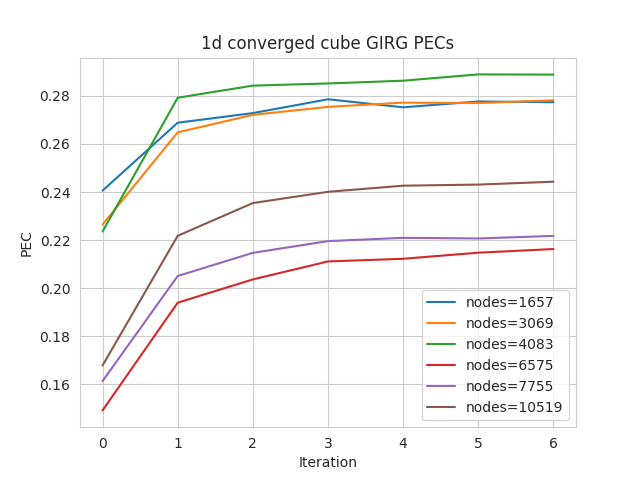
\includegraphics[width=0.49\textwidth]{figures/mcmc_ordered_1d_pec_convergence.png}
  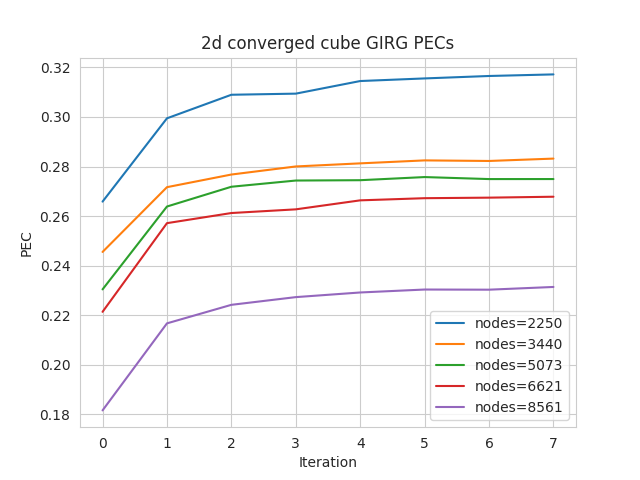
\includegraphics[width=0.49\textwidth]{figures/mcmc_ordered_2d_pec_convergence.png}
  \caption{Direct ordered likelihood maximisation PEC convergence over iterations for some example socfb graphs.}
  \label{fig:direct_ordered_pec_convergence_curves}
\end{figure}


\begin{figure}
  \centering
  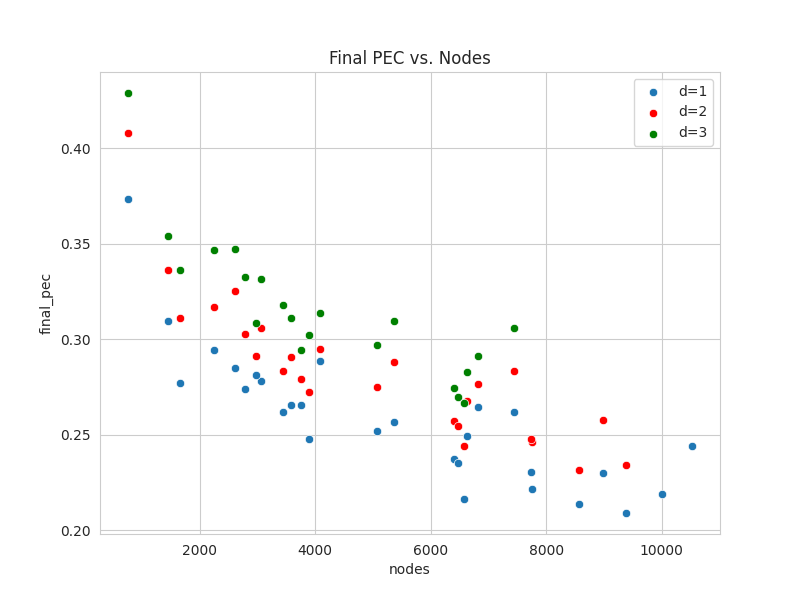
\includegraphics[width=\textwidth]{figures/mcmc_ordered_final_pec.png}
  \caption{converged PECs for 1d, 2d, 3d cube GIRGs. Missing some 3d numbers
  as batch job exceeded allotted time.}
  \label{fig:converged_pecs}
\end{figure}


TODO further improvements might be: updating weight estimates (adding into ordered MCMC, as per mercator). Making code run on GPU.


\begin{figure}
  \caption{2d cube GIRG fitting examples: Two diffusion map embeddings with different post-processing methods The blue lines for the restricted version show the border at which points are outer uniformified. Then heat map / scatter plot for further refined point locations using direct ordered likelihood maximisation.}
  \label{fig:uniformifed_vs_restricted_rescaling}
  \centering

  \begin{subfigure}{\textwidth}
    \centering
    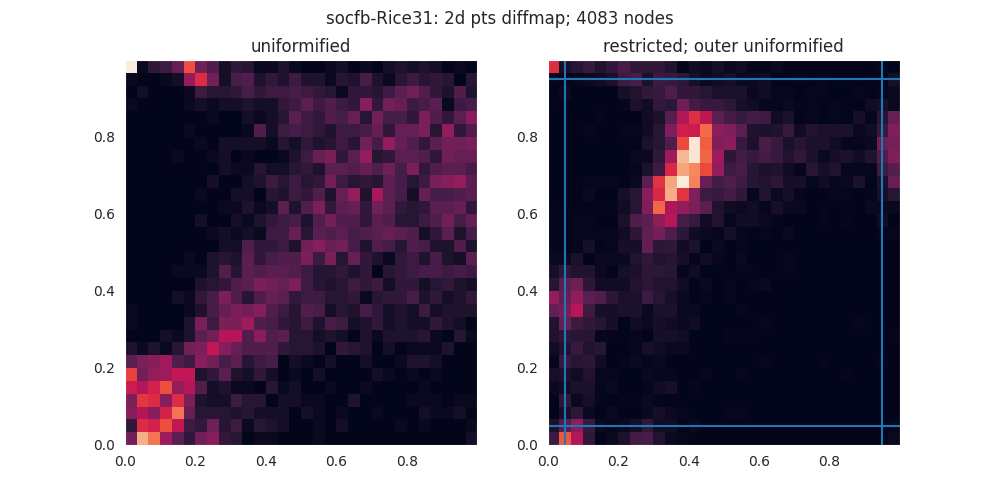
\includegraphics[width=\linewidth]{figures/socfb-Rice31_2ddiffmap_unif_vs_restrict.png}
    % \label{fig:sub1}
  \end{subfigure}

  \vspace{1em}
  \begin{subfigure}{\textwidth}
    \centering
    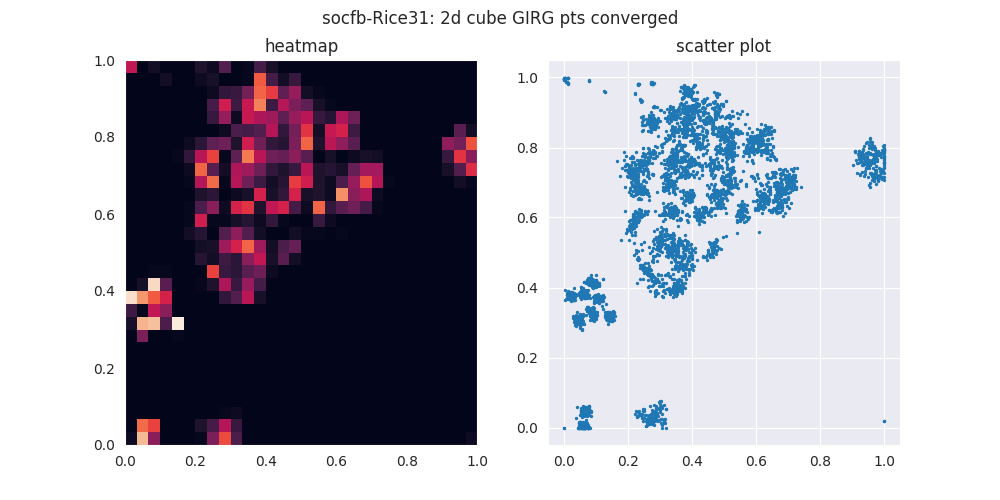
\includegraphics[width=\linewidth]{figures/socfb-Rice31_2d_cube_GIRG_converged.png}
    % \label{fig:sub1}
  \end{subfigure}

  \vspace{1em}
  
\end{figure}
\begin{figure}
  \begin{subfigure}{\textwidth}
    \centering
    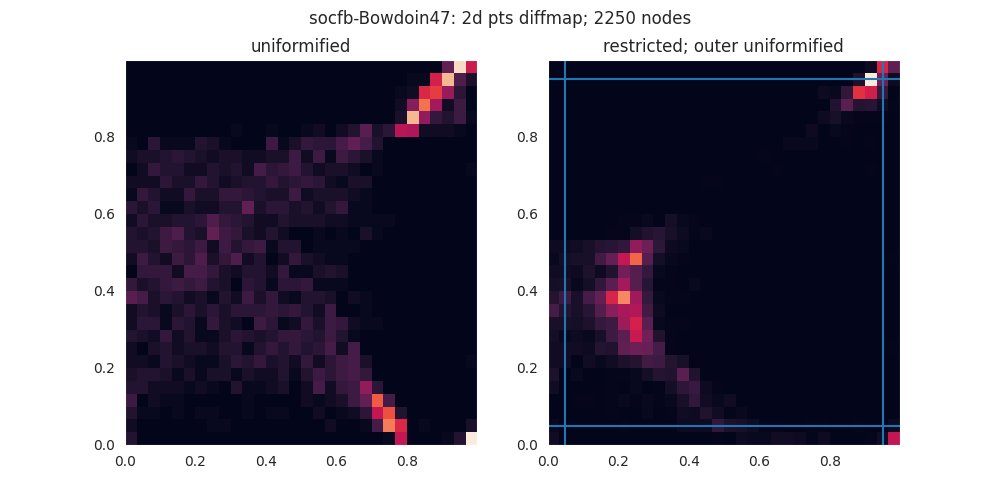
\includegraphics[width=\linewidth]{figures/socfb-Bowdoin47_2ddiffmap_unif_vs_restrict.png}
    % \label{fig:sub1}
  \end{subfigure}

  \vspace{1em}
  \begin{subfigure}{\textwidth}
    \centering
    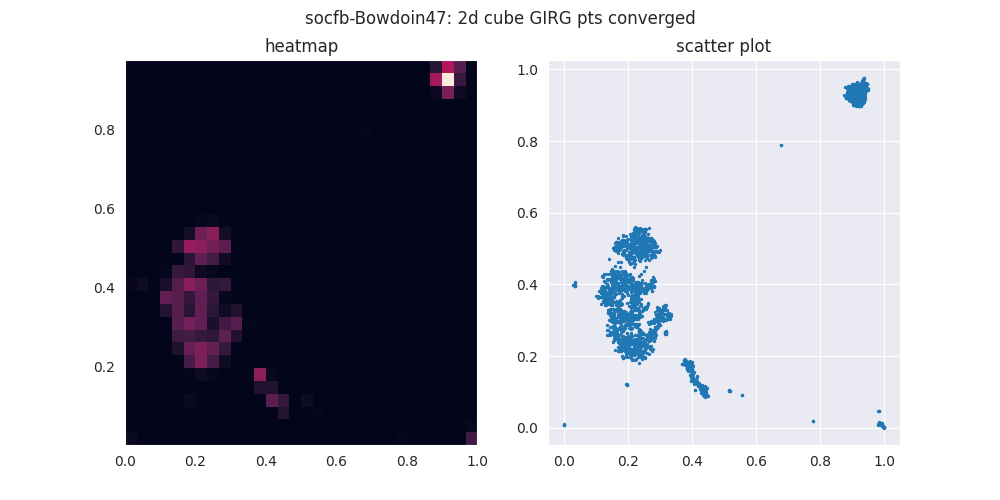
\includegraphics[width=\linewidth]{figures/socfb-Bowdoin47_2d_cube_GIRG_converged.png}
    % \label{fig:sub1}
  \end{subfigure}

\end{figure}

\begin{figure}
  \begin{subfigure}{\textwidth}
    \centering
    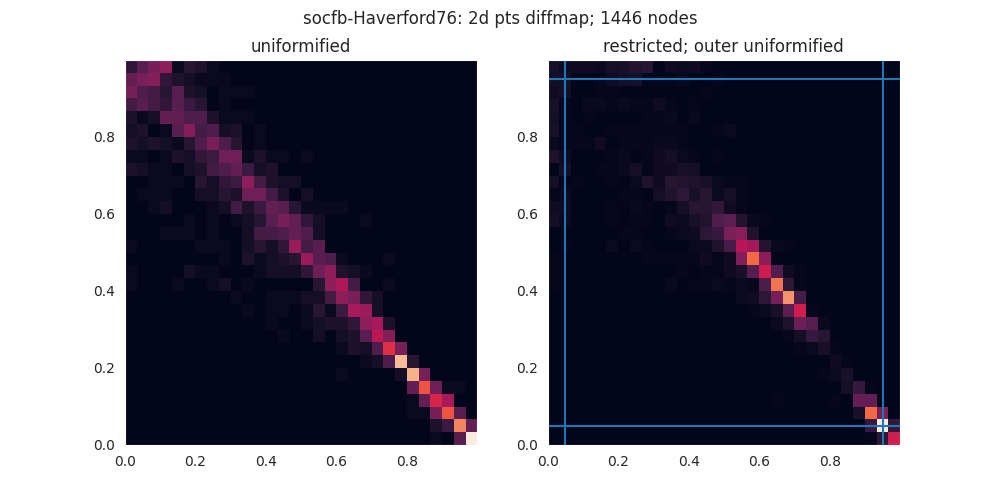
\includegraphics[width=\linewidth]{figures/socfb-Haverford76_2ddiffmap_unif_vs_restrict.png}
    % \label{fig:sub1}
  \end{subfigure}

  \vspace{1em}
  \begin{subfigure}{\textwidth}
    \centering
    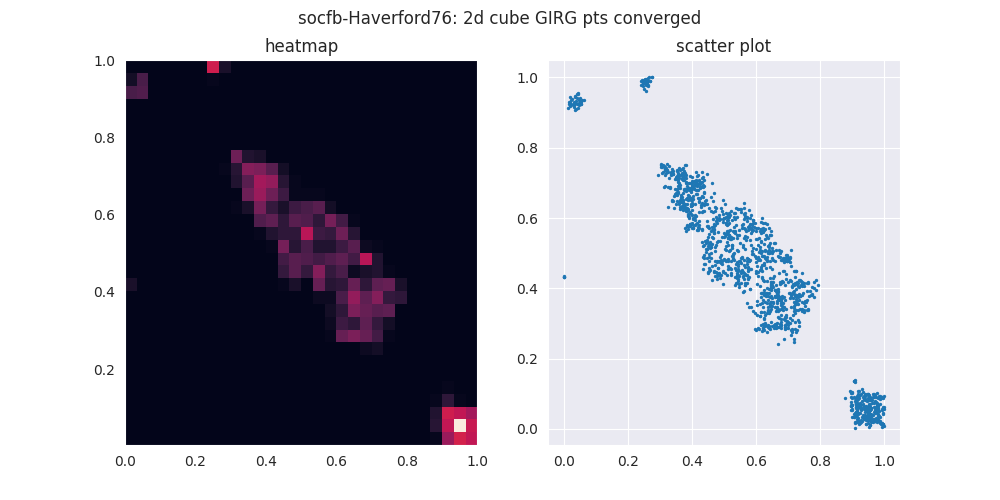
\includegraphics[width=\linewidth]{figures/socfb-Haverford76_2d_cube_GIRG_converged.png}
    % \label{fig:sub1}
  \end{subfigure}

\end{figure}


% \subsection{point initalisation and failure rate}
% Initially I ran MCMC using uniformified diffusion map initialisation, and failure rate $0.0$. The MCMC would converge, but actually take longer than necessary, as the "good" initialisation was being undone in favour of quite spaced out points.

% The evidence for this is shown in some plots of points over time:

% \begin{figure}
%   \centering
%   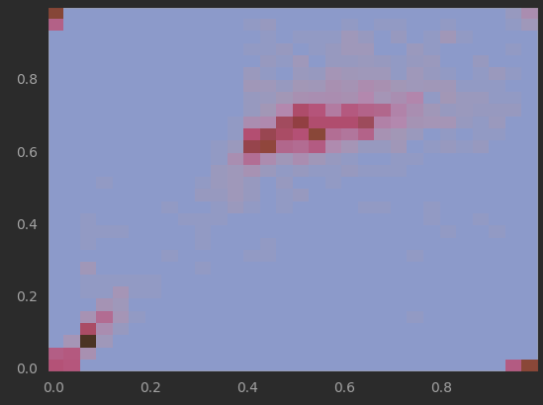
\includegraphics[width=\textwidth]{figures/amherst_2d_pts_restricted.png}
%   \caption{0.05 quantile restricted and uniformed at the edges diffusion map initialisation of MCMC points for socfb-Amherst41}
% \end{figure}

% \begin{figure}

%   \begin{subfigure}{1.0\textwidth}
%   \centering
%   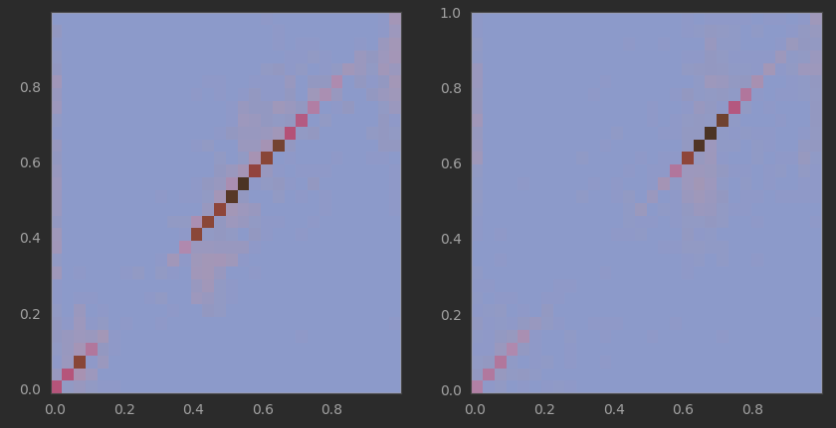
\includegraphics[width=\linewidth]{figures/amherst_failure_mcmc_pts.png}
%   \caption{failure rate $0.3$}
% \end{subfigure}

%   \vspace{1em}

%   \begin{subfigure}{1.0\textwidth}
%   \centering
%   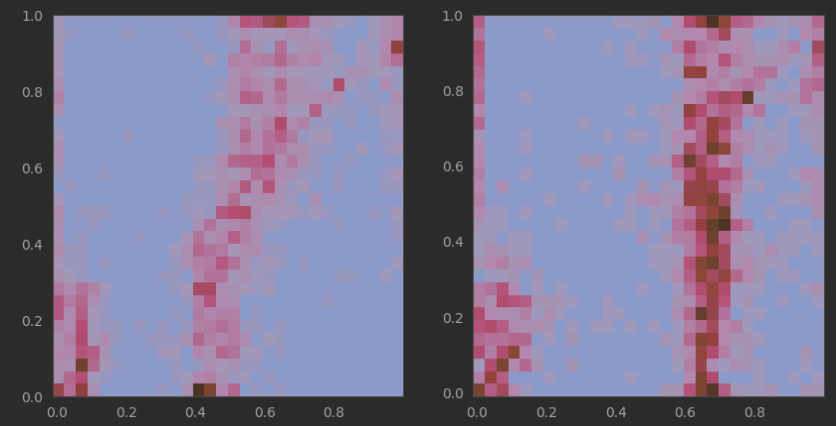
\includegraphics[width=\linewidth]{figures/amherst_nonfailure_mcmc_pts.png}
%   \caption{failure rate $0.0$ (aka no failure rate)}
% \end{subfigure}

%   \caption{MCMC iterated points scatter plot against initialisation, with/without failure rate}
%   \label{fig:amherst_points_over_time}
% \end{figure}


% Run long enough, the MCMC's points converge to the cube:

% \begin{figure}
%   \centering
%   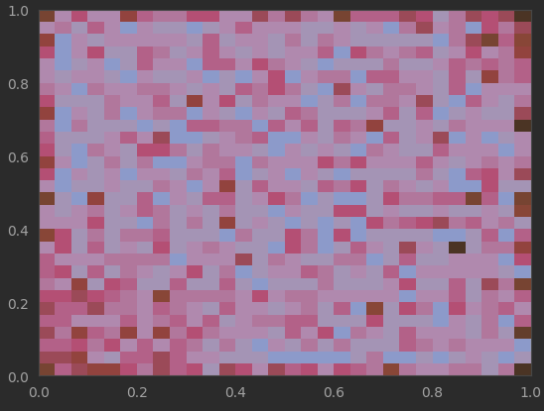
\includegraphics[width=\textwidth]{figures/MCMC_converged_to_cube.png}
%   \caption{failure rate $0.0$ run until convergence for 2D GIRG: points 2D histogram}
% \end{figure}


% \begin{table}[ht]
%   \centering
%   \begin{tabular}{|l|l|}
%   \hline
%   \textbf{LL maximum for 1D} & \textbf{LL maximum for 2D} \\
%   \hline
%   socfb-Amherst41 & socfb-Bowdoin47 \\
%   socfb-Oberlin44 & socfb-Caltech36 \\
%   socfb-Reed98 & socfb-Colgate88 \\
%   socfb-Swarthmore42 & socfb-Hamilton46 \\
%   socfb-Wellesley22 & socfb-Haverford76 \\
%   & socfb-Middlebury45 \\
%   & socfb-Pepperdine86 \\
%   & socfb-Santa74 \\
%   & socfb-Simmons81 \\
%   & socfb-Smith60 \\
%   & socfb-Trinity100 \\
%   & socfb-USFCA72 \\
%   & socfb-Vassar85 \\
%   & socfb-Williams40 \\
%   \hline
%   \end{tabular}
%   \caption{Your Caption}
%   \label{tab:my_label}
%   \end{table}




